\subsection*{Timing}

\begin{figure}[h]
\begin{centering}
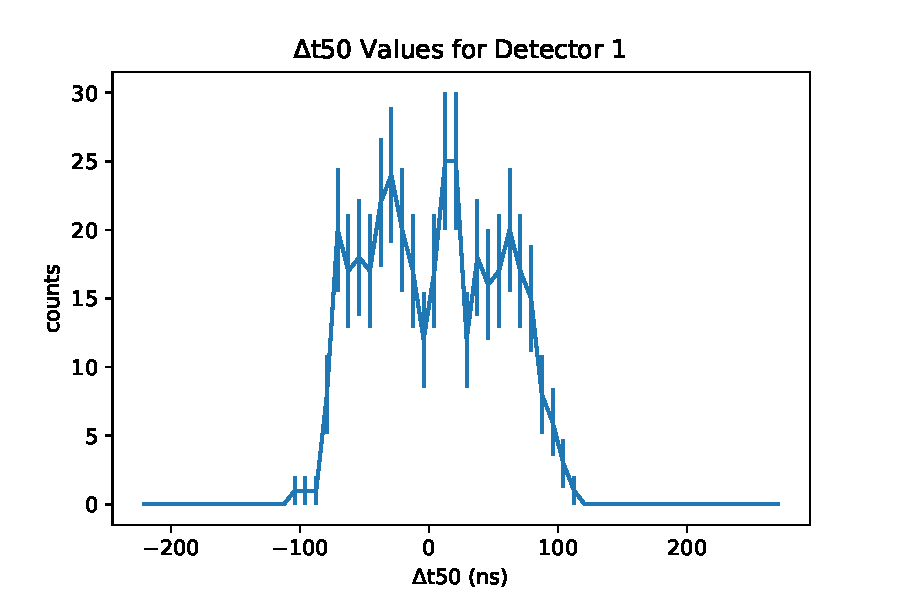
\includegraphics[width=0.7\textwidth]{./figures/t50s_det1.pdf}
\caption{The $\Delta t50$ distribution for detector 1.}
\label{t50_1}
\end{centering}
\end{figure}

Plotted is the distribution of $\Delta t50$ for both detectors. The source was located on the DC side of detector1. Events close to this face correspond to the most negative values of $\Delta t50$. We expect to see an exponential fall-off of events as depth increases from this point. There is some exponential trend, however, at the opposite side of the detector 

\begin{figure}[h]
\begin{centering}
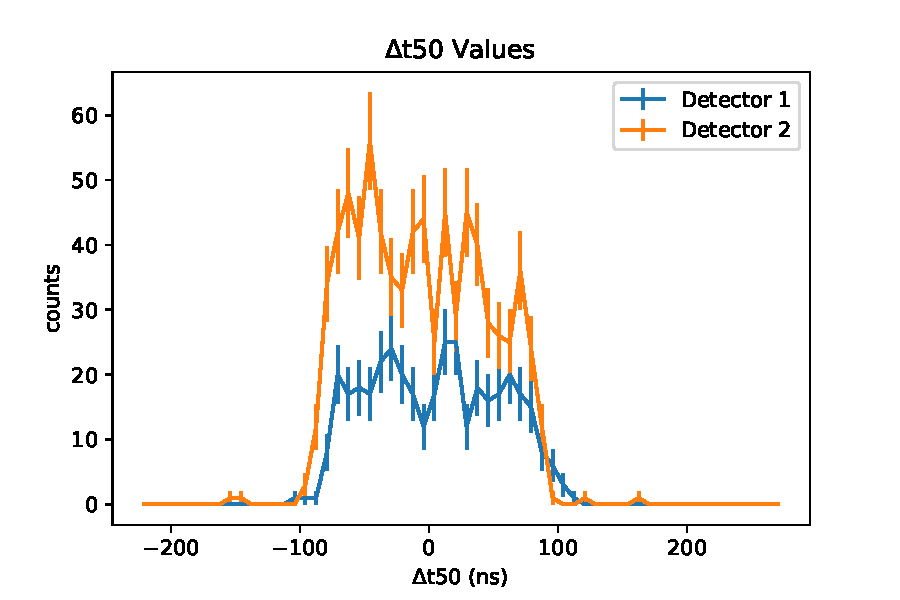
\includegraphics[width=0.7\textwidth]{./figures/t50s_det2.pdf}
\caption{The $\Delta t50$ distribution for detector 2.}
\label{t50_2}
\end{centering}
\end{figure}

The trigger time of a signal is determined by a on-board fast trapezoidal shaper. This trigger time may differ slightly between signals, depending on the location of the interaction, leading to additional uncertainty. The effect of this jitter will be studied for more precise position determination.

\subsection*{Depth Determination}

-depth profile with theoretical curve for comparison

\begin{figure}[h]
\begin{centering}
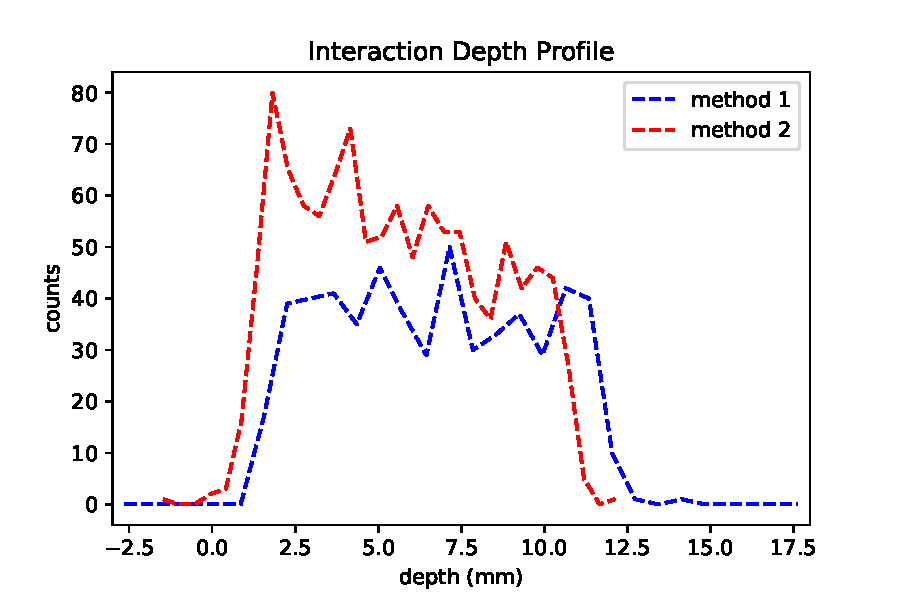
\includegraphics[width=0.7\textwidth]{./figures/interactiondepths.pdf}
\caption{The $\Delta t50$ distribution for detector 2.}
\label{t50_2}
\end{centering}
\end{figure}

The depth profile for detector 1 is shown in \ref{interactiondepths}. The second method of calculating depth, which takes into account the different carrier velocities, seems to give a better result. More events are confined within the detector and the depth profile looks to have a stronger exponential trend.

Some events will be subject to charge sharing, charge loss in the inter-strip gap, collection to a disconnected strip, etc. If the total charge gathered on one side of the detector by the main collecting electrode is not great enough, the signal may not be recorded. This leads to 

Another source of error is scattering events. A gamma ray may scatter in an event with full-energy deposition (forward Compton scattering within a voxel for example), and the assumption of a single scattering event where there were two or more will lead to an improperly reconstructed interaction position. This is another source of error in our measurement. However, with the Geant4 data, we have determined that 

\subsection*{Comparison to Simulation}

A simple model was built in GEANT4 (two planar HPGe crystals, 74 mm wide, 15 mm thick, 10 mm apart). No surrounding material was included in the model. A point source emitting gamma-rays with energy 661.657 keV from a point 2 meters in front of the front-face of the first detector was used \cite{ebss}. This data was used to compare to the experimentally determined distribution of interaction depths.